\documentclass[12pt]{article}
\usepackage{graphicx}
\usepackage{multirow}
\usepackage{longtable}
\usepackage{listings}
\usepackage[letterpaper, margin=2cm]{geometry}
\usepackage[T1]{fontenc}
\usepackage{polski}
\usepackage[export]{adjustbox}
\usepackage[utf8]{inputenc}
\usepackage[polish]{babel}
\graphicspath{{.}}
\usepackage{tocloft}
\usepackage{hyperref}

\hypersetup{%
    colorlinks,
    citecolor=black,
    filecolor=black,
    linkcolor=black,
    urlcolor=black
}

\renewcommand{\cftsecleader}{\cftdotfill{\cftdotsep}}

\lstset{
    postbreak=\mbox{\textcolor{red}{$\hookrightarrow$}\space}
    belowcaptionskip=1\baselineskip,
    breaklines=true,
    frame=L,
    numbers=left,
    xleftmargin=\parindent,
    language=bash,
    showstringspaces=false,
    basicstyle=\footnotesize\ttfamily,
    identifierstyle=\color{blue},
    stringstyle=\color{orange},
}

\begin{document}
    \centering
    
\includegraphics[width=5cm, height=5cm,]{herbPL.jpg}
    \hspace{2cm}
    
\includegraphics[width=5cm, height=5cm]{herbWEII.jpg}\\
    \vspace{2cm}
    {\Huge \textbf{SPRAWOZDANIE}}
    \vspace{2cm}
    \newline
    {\large PROJEKTOWANIE INTERFEJSÓW I ERGONOMIA SYSTEMÓW}
    \vfill
    \raggedright
    \textbf{IMIĘ I NAZWISKO:} Piotr Czajka

    \textbf{NUMER LABORATORIUM} 3\\
    \textbf{GRUPA:} 7.1.2\\
    \textbf{Data wykonywania ćwiczenia:} 02.11.2018\\

    \newpage

    \tableofcontents{}

    \newpage

    \section{Cel laboratorium}
    Celem laboratorium było zapoznanie się z tematem interfejsów mobilnych, problemami ich ergonomii i jakości

    \section{Przebieg ćwiczenia}

    \subsection{Zadanie 3.1. Ocena możliwości personalizacji mobilnego systemu operacyjnego}

    Wylicz elementy umożliwiajace personalizacje systemu operacyjnego w Twoim telefonie

    \begin{longtable}{|p{0.33\textwidth}|p{0.33\textwidth}|p{0.33\textwidth}|}
        \cline{1-2}
        \textbf{Typ telefonu:} & Xiaomi Redmi Note 4 \\
        \cline{1-2}
        \textbf{System operacyjny:} & Lineage OS (Android based)\\
        \hline
        \textbf{Możliwość personalizacji} & \textbf{Zakres personalizacji} & \textbf{Uwagi/Zrzuty ekranu}\\
        \hline
        1. Zmiana rozmiaru czcionki systemowej & dostępnych jest kilka stopni wyboru wielkości czcionki & 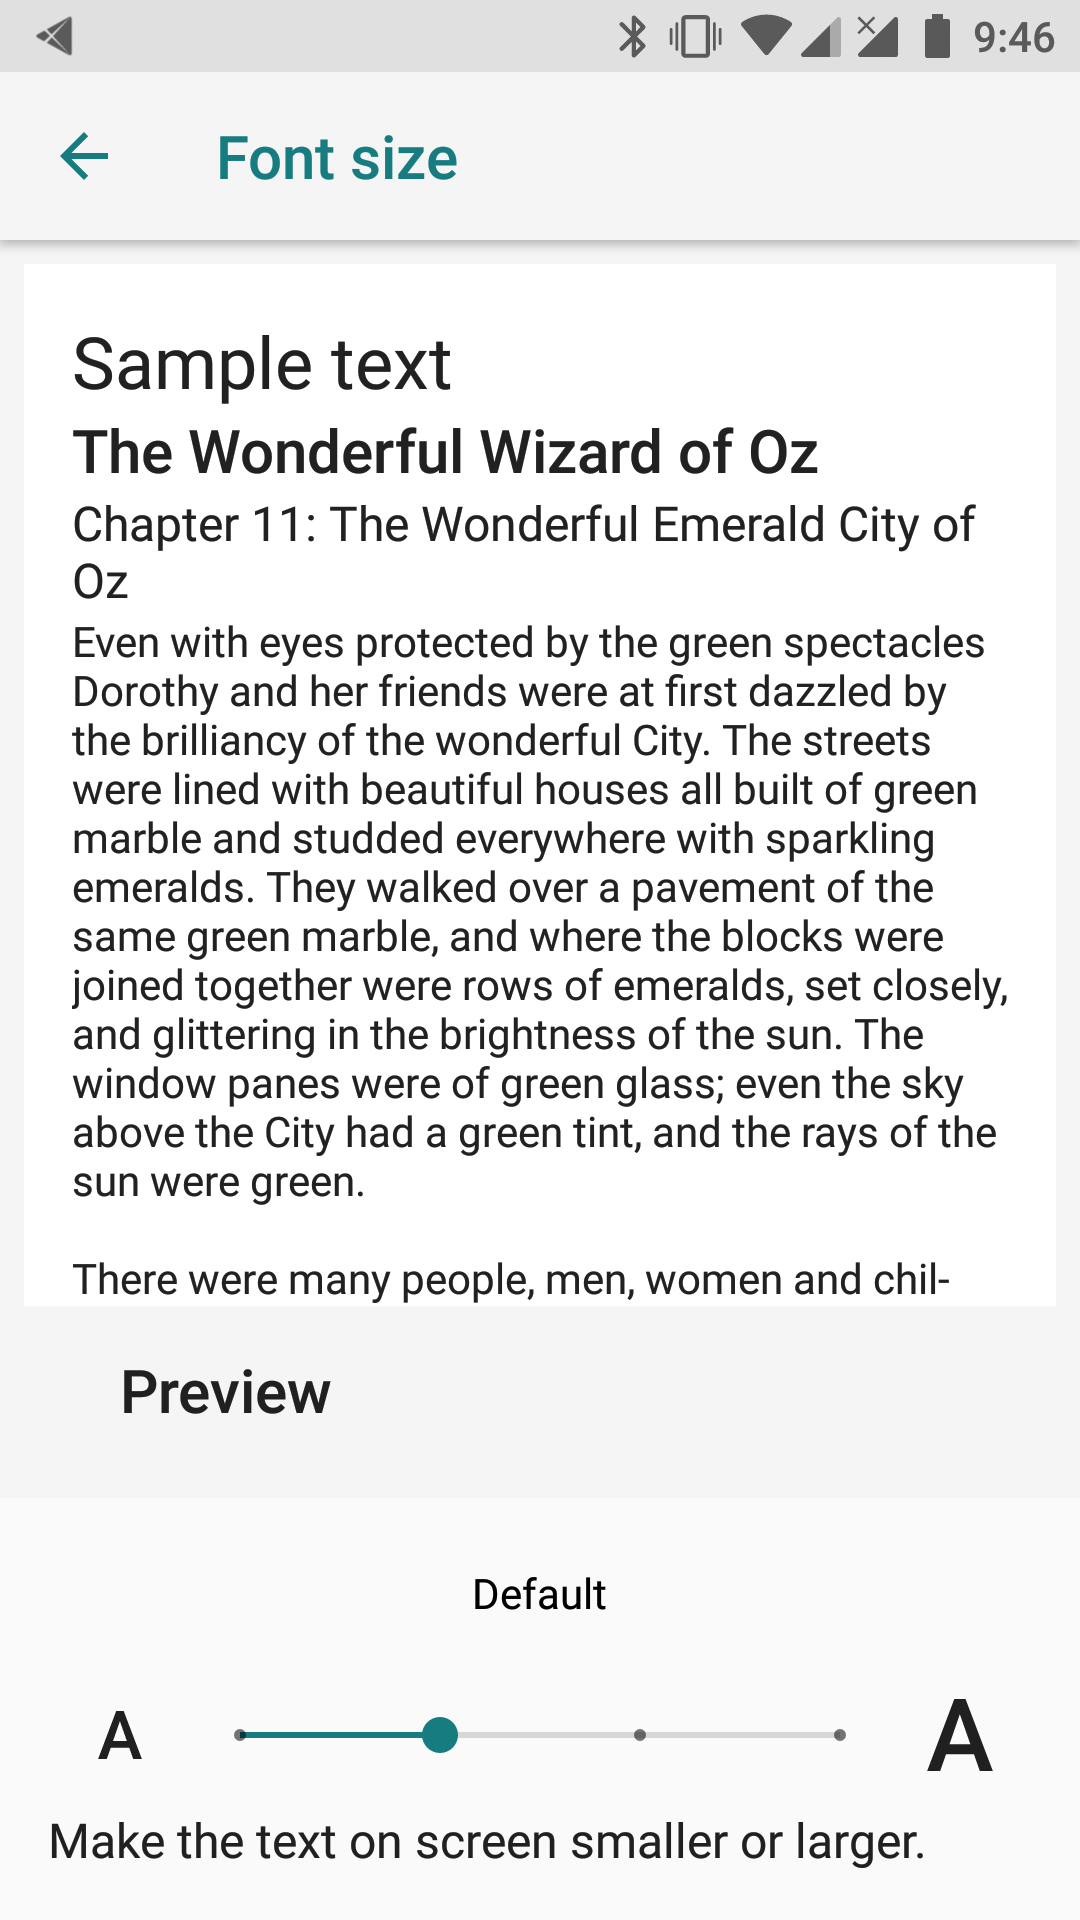
\includegraphics[scale=0.1]{changefont.png}\\
        \hline
        2. Persolnalizacja ekranu głównego & Poza dowolnym rozmieszczaniem ikon na ekranie, dodawaniu i usuwaniu ekranów istnieje też możliwość dodawania na ekran nowych widgetów i ustawiania tapet & 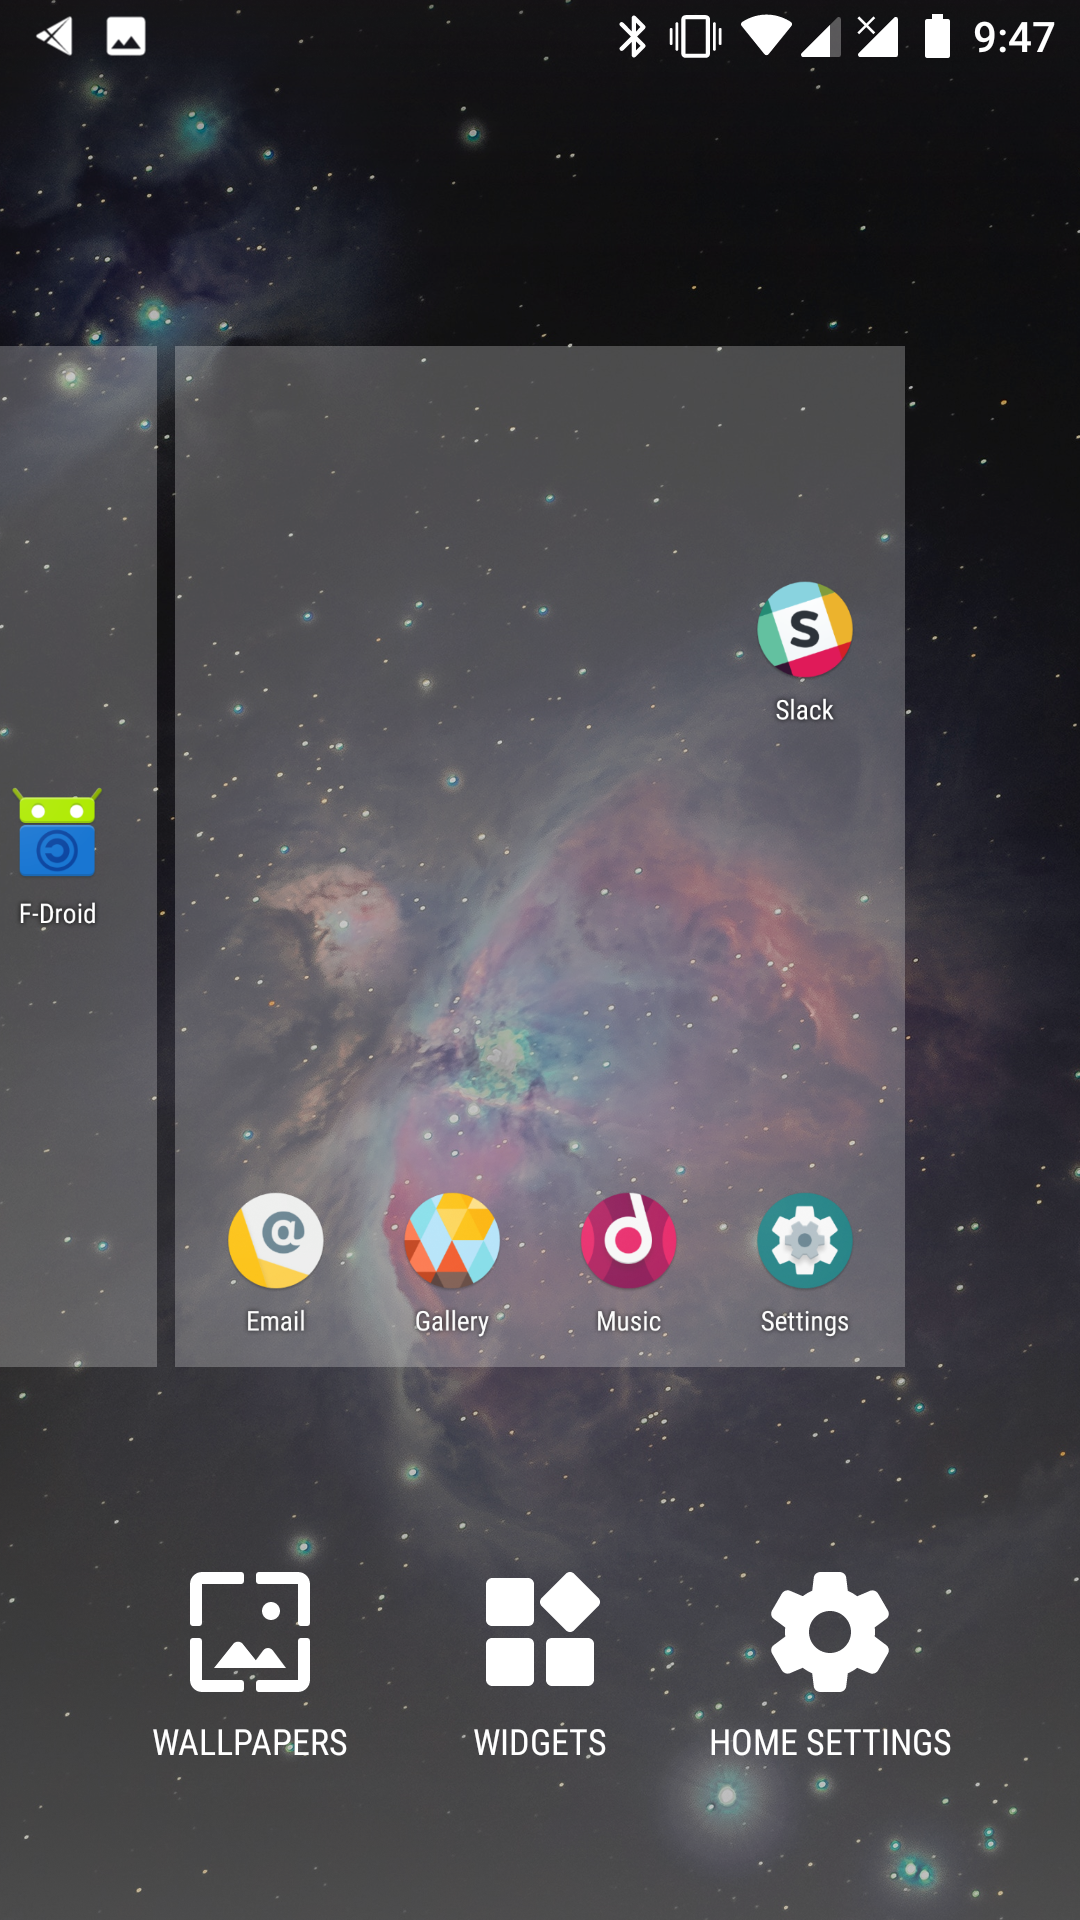
\includegraphics[scale=0.1]{changedesktop.png}\\
        \hline
        3. Personalizacja wysuwanego z góry menu & Możliwym jest dodawanie nowych ikon na pasek wysuwany z góry, spośród skończonej puli gotwych kontrolek. Można też dowolnie usuwać/przesuwać kontrolki & 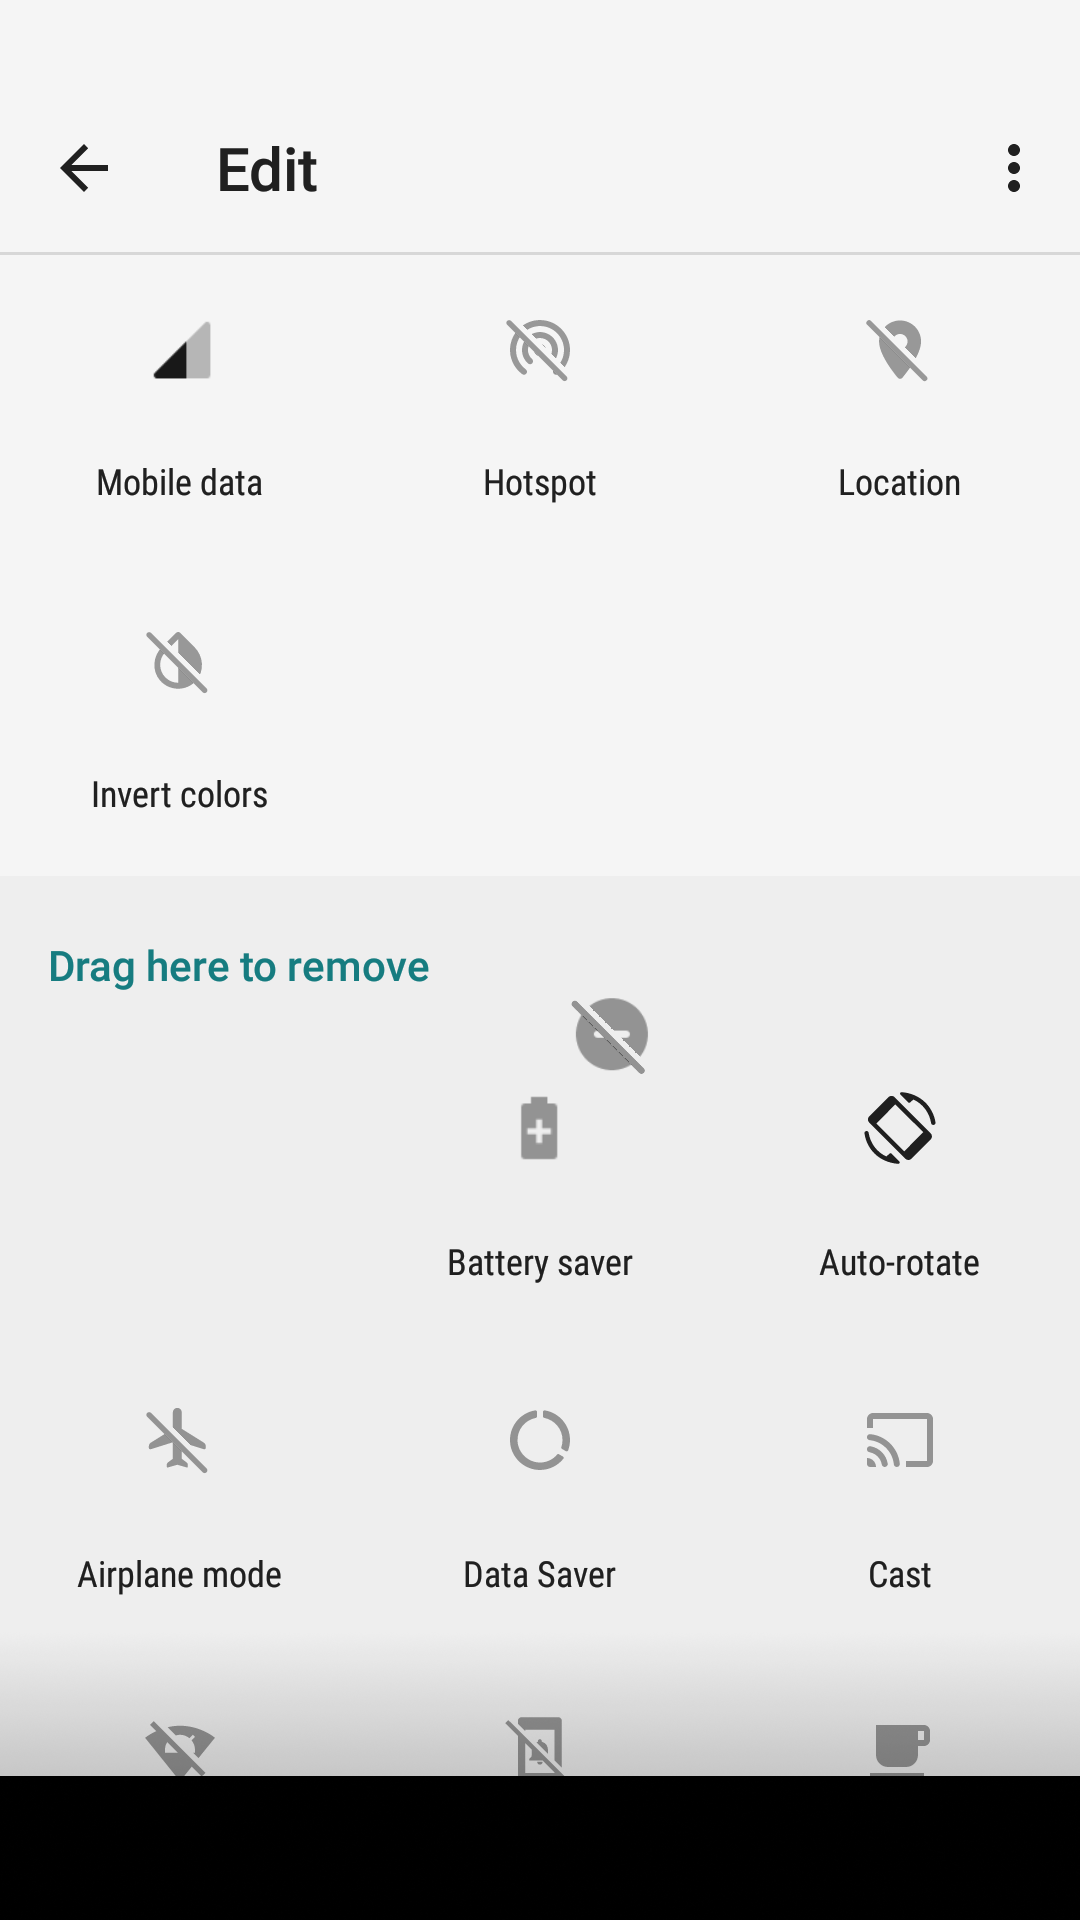
\includegraphics[scale=0.1]{changemenu.png}\\
        \hline
        4. Możliwość zmiany barwy światła & Umożliwienie regulacji ilości niebieskiego światła, jakie jest emitowane przez urządzenie, z podziałem na noc i na dzień & 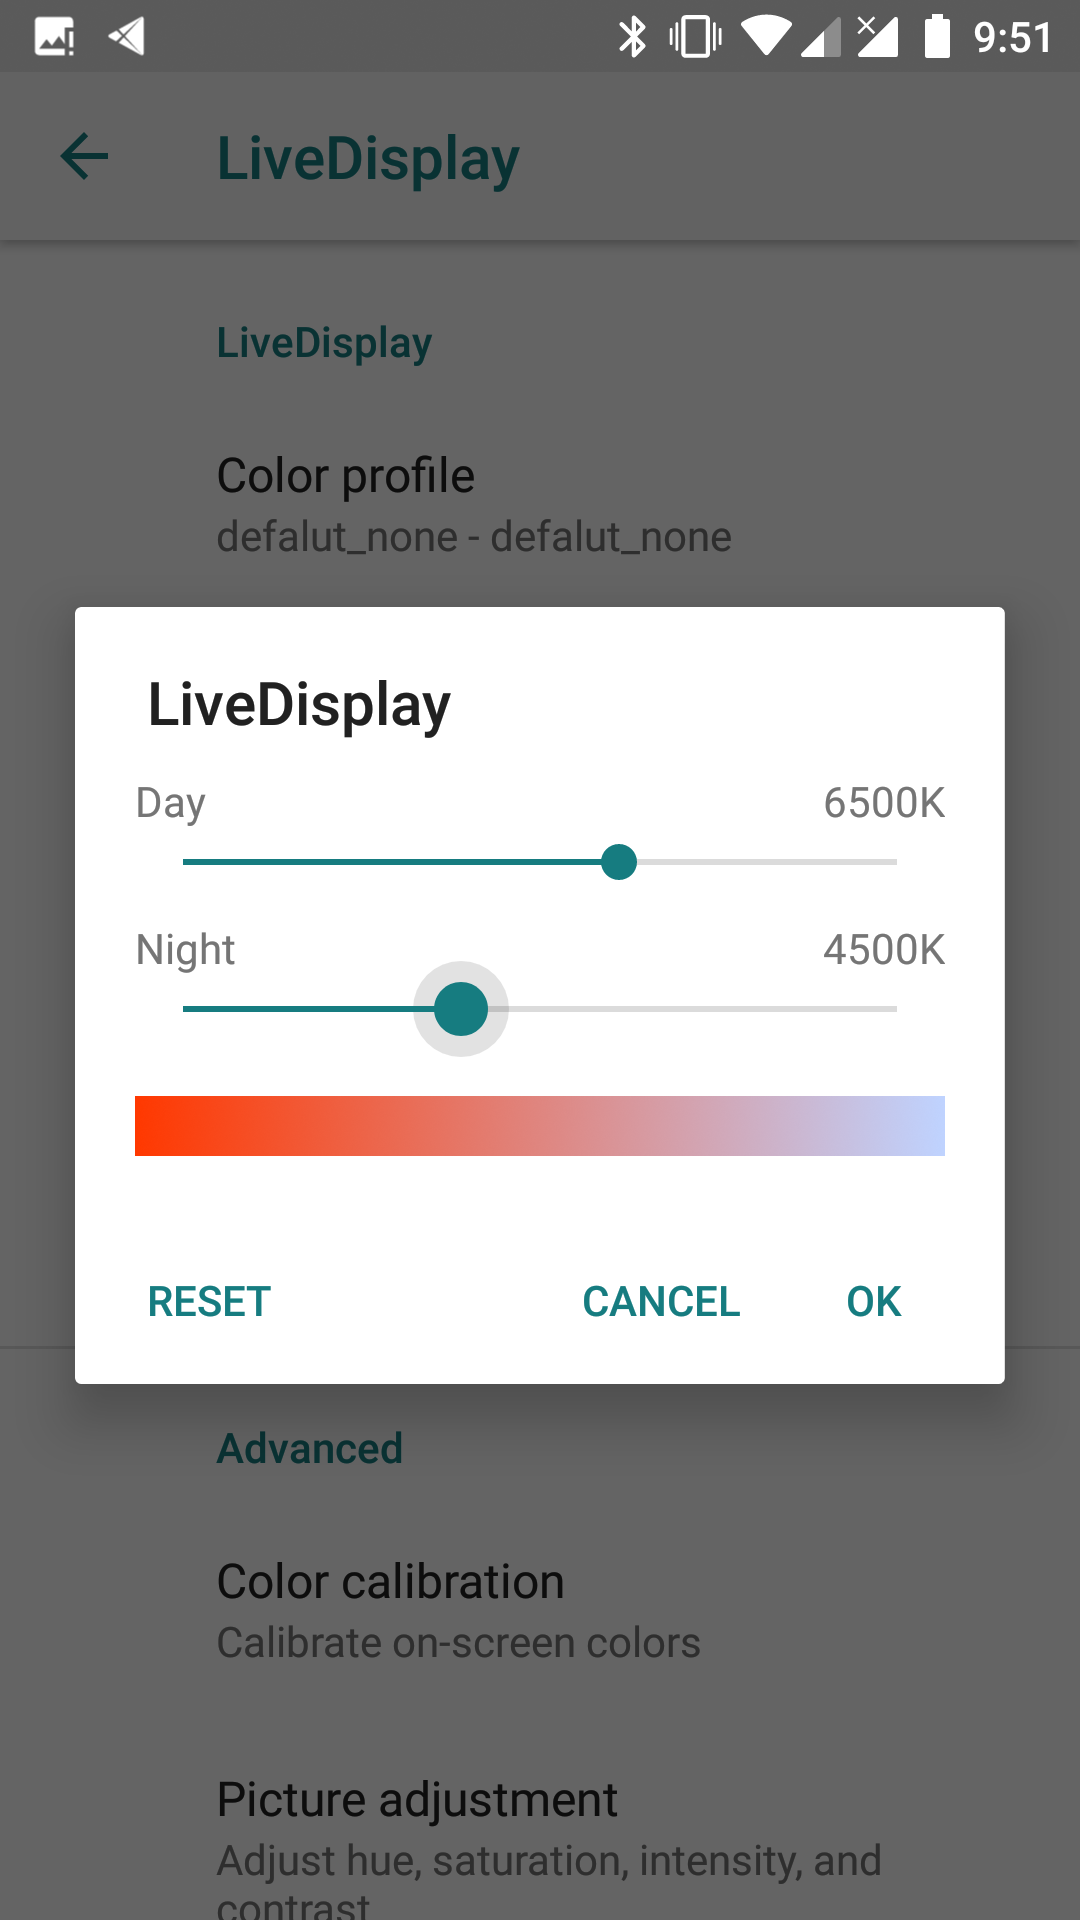
\includegraphics[scale=0.1]{changetemp.png}\\
        \hline
        5. Możliwość zmiany nazw ikon & Każda podpisana ikona w systemie ma dodatkową możliwość nadania jej innej nazwy poprzez jej przytrzymanie i późniejsze wpisanie żądanej nazwy& 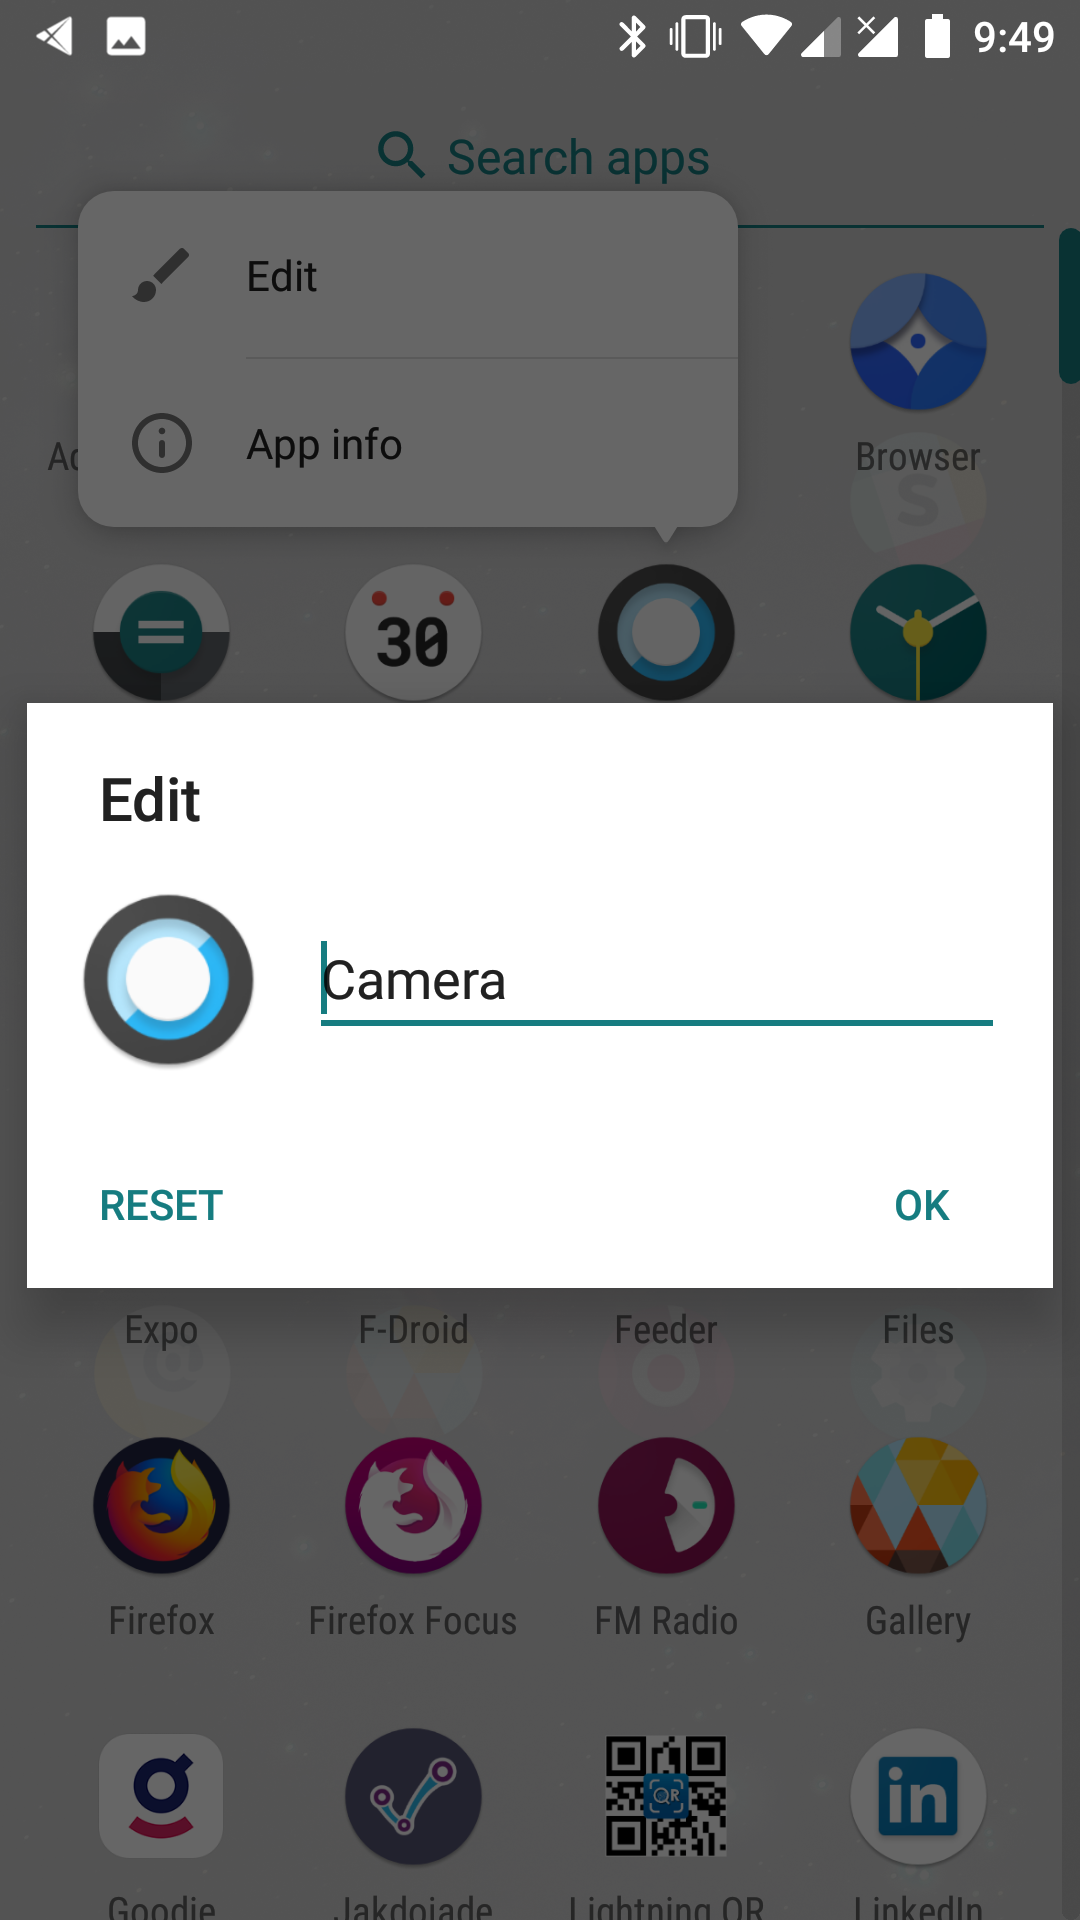
\includegraphics[scale=0.1]{changename.png}\\
        \hline
    \end{longtable}

    \subsection{Zadanie 3.2. Ocena możliwości użycia gestów}

    Wylicz, jakie gesty są dostępne w Twoim telefonie dla 3 aplikacji. Postaraj się, by były one różne.

    \begin{longtable}{|p{0.5\textwidth}|p{0.5\textwidth}|}
        \hline
        \textbf{Typ telefonu:} & Xiaomi Redmi Note 4\\
        \hline
        \textbf{System operacyjny:} & Lineage OS (Android based)\\
        \hline
        \textbf{Nazwa aplikacji} & \textbf{Gesty oraz interakcje}\\
        1. Jak dojadę & \textbf{Scroll} przy przewijaniu rozkładu \textbf{Pinch} i \textbf{Zoom} przy przeglądaniu mapy.\\
        2. Protonmail & \textbf{Flick} przy kasowaniu maili, lub oznaczaniu ich jako odczytane\\
        3. Phone & \textbf{Long Press} do rozwinięcia menu kontekstowego dla danego numeru, \textbf{tap} do wybrania numeru i \textbf{flick} do odebrania/zignorowania połączenia przychodzącego\\
    \end{longtable}

    \subsection{Zadanie 3.3 Jakość aplikacji mobilnej}

    Oceń jakość posiadanej aplikacji mobilnej (np. wyświetlacjącej prognozę pogody lub budzika.

    \begin{longtable}{|p{0.4\textwidth}|p{0.1\textwidth}|p{0.5\textwidth}|}
        \cline{1-2}
        \textbf{Typ telefonu:} & Xiaomi Redmi Note 4\\
        \cline{1-2}
        \textbf{Aplikacja:} & Clock\\
        \hline
        Obszar & Ocena & Uzasadnienie\\
        \hline
        1. Nawigacja & 5/5 & 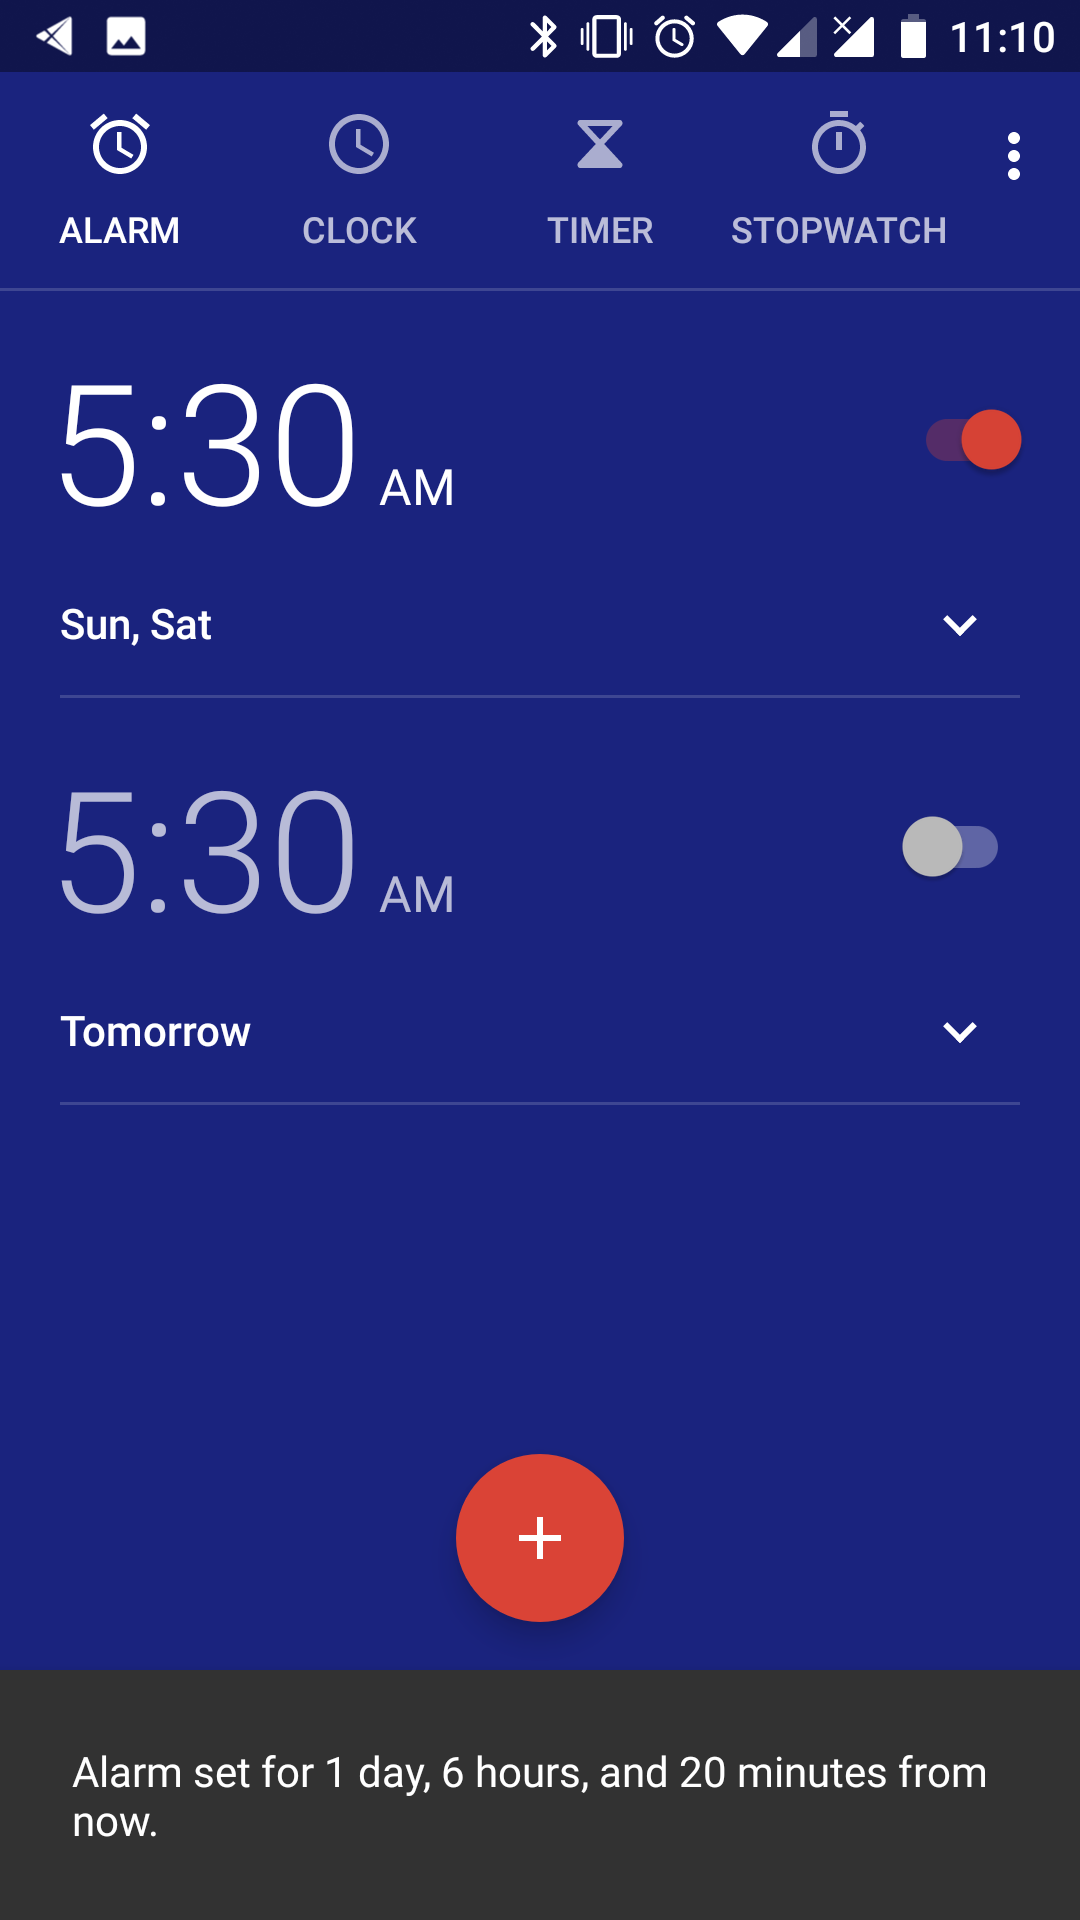
\includegraphics[scale=0.1]{alarmset.png} Nawigacja jest w aplikacji wykonana intuicyjnie, na górze mamy czytelne menu z ikonami, które prowadzą nas do konkretnych funkcji zegara. Strzałka w tył w tym przypadku po prostu wychodzi z aplikacji, ponieważ nie posiada ona żadnej sekwencji ekranów, w której sensownie byłoby się móc cofać. Do nawigacji wykorzystane są podstawowe gesty takie jak: tap, scroll. Scroll służy do przewijania ew. listy alarmów, lub przewijania listy "zegary świata".\\
        \hline
        2. Informacja zwrotna & 4/5 & 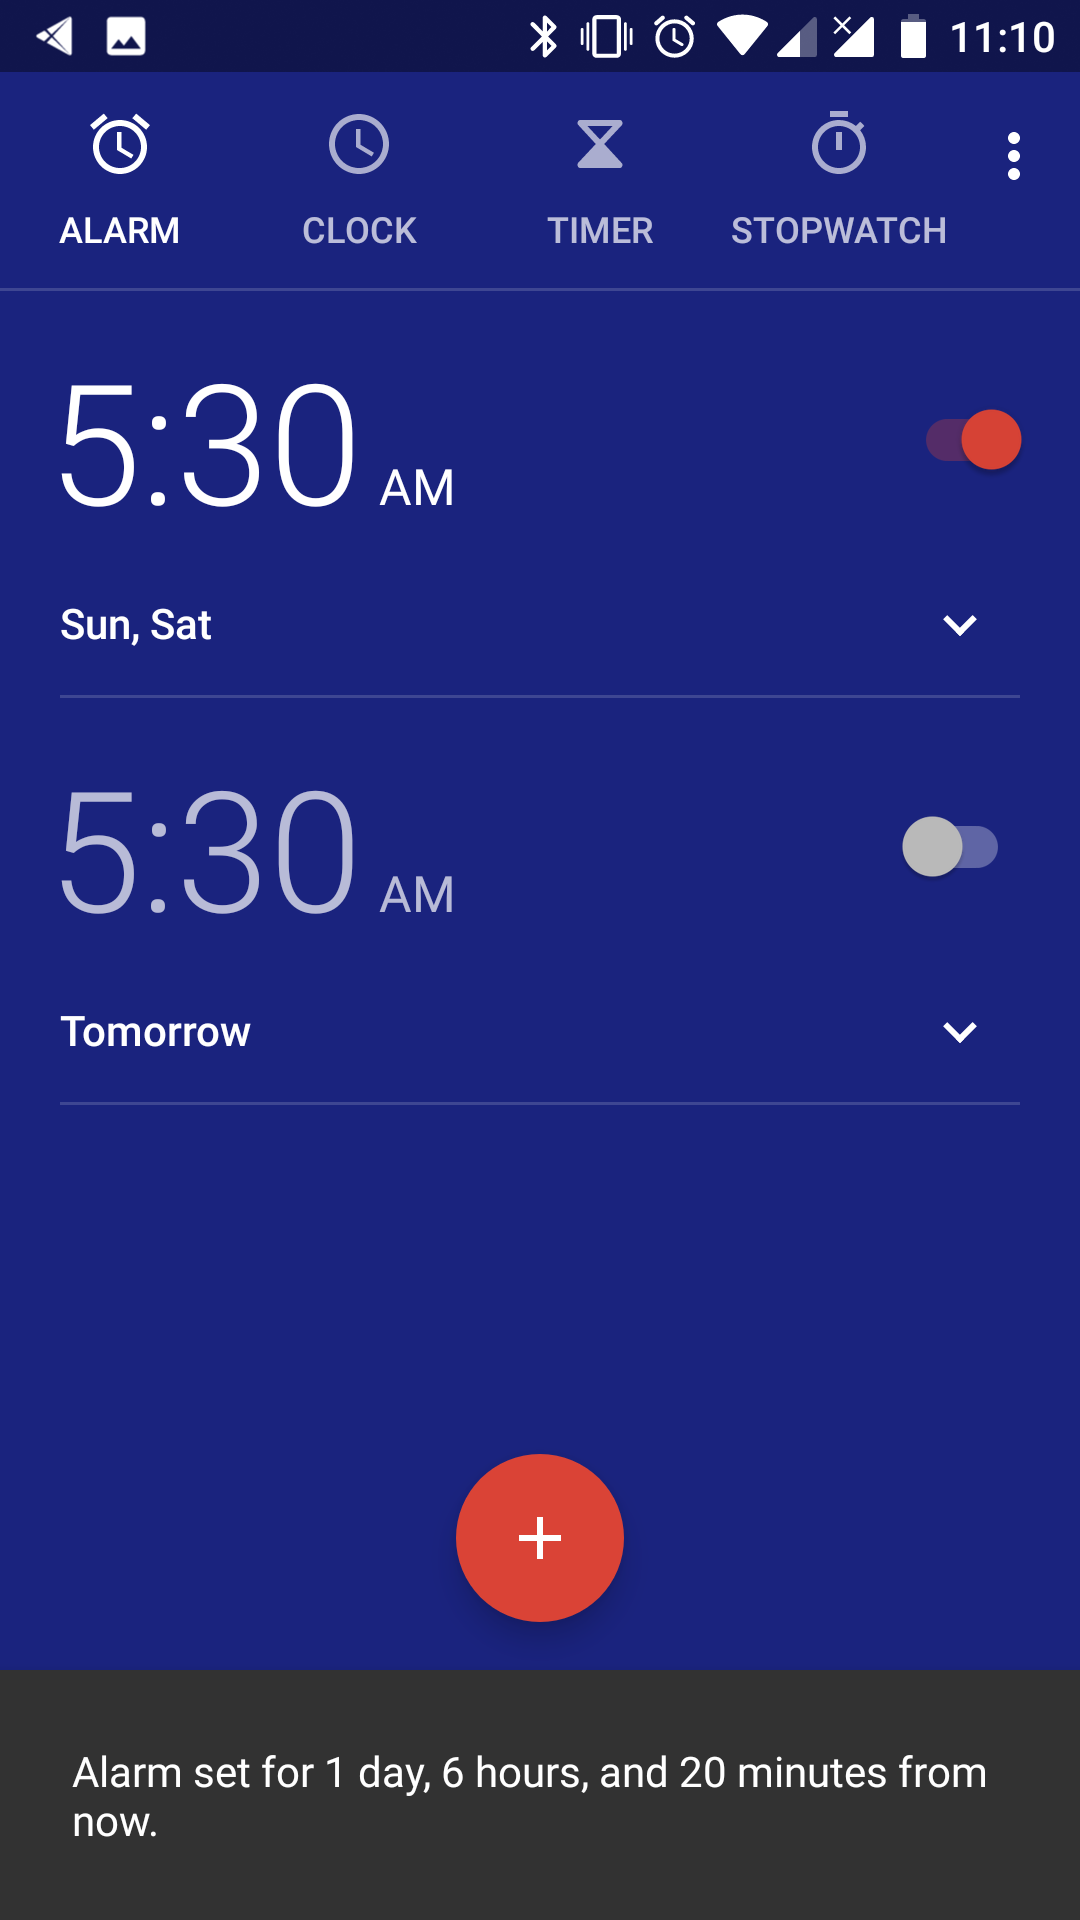
\includegraphics[scale=0.1]{alarmset.png} Po wykonaniu postawowych akcji, takiej jak na przykład nastawienie budzika, dostajemy od aplikacji informacje zwrotną w postaci tekstowego popupu wyświetlającego się na dole ekranu. Mamy po za tym też widocznego na ekranie slidera, który przesunął i podświetlił się, symbolizując włączenie alarmu. Tekstowe informacje są czytelne, jednak nie zawsze są one idealnym rozwiązaniem. Szczególnie w przypadku osoby niedowidzącej, dlatego ocena jest odpowiednio mniejsza.\\
        \hline
        3. Konsekwencja & 5/5 & 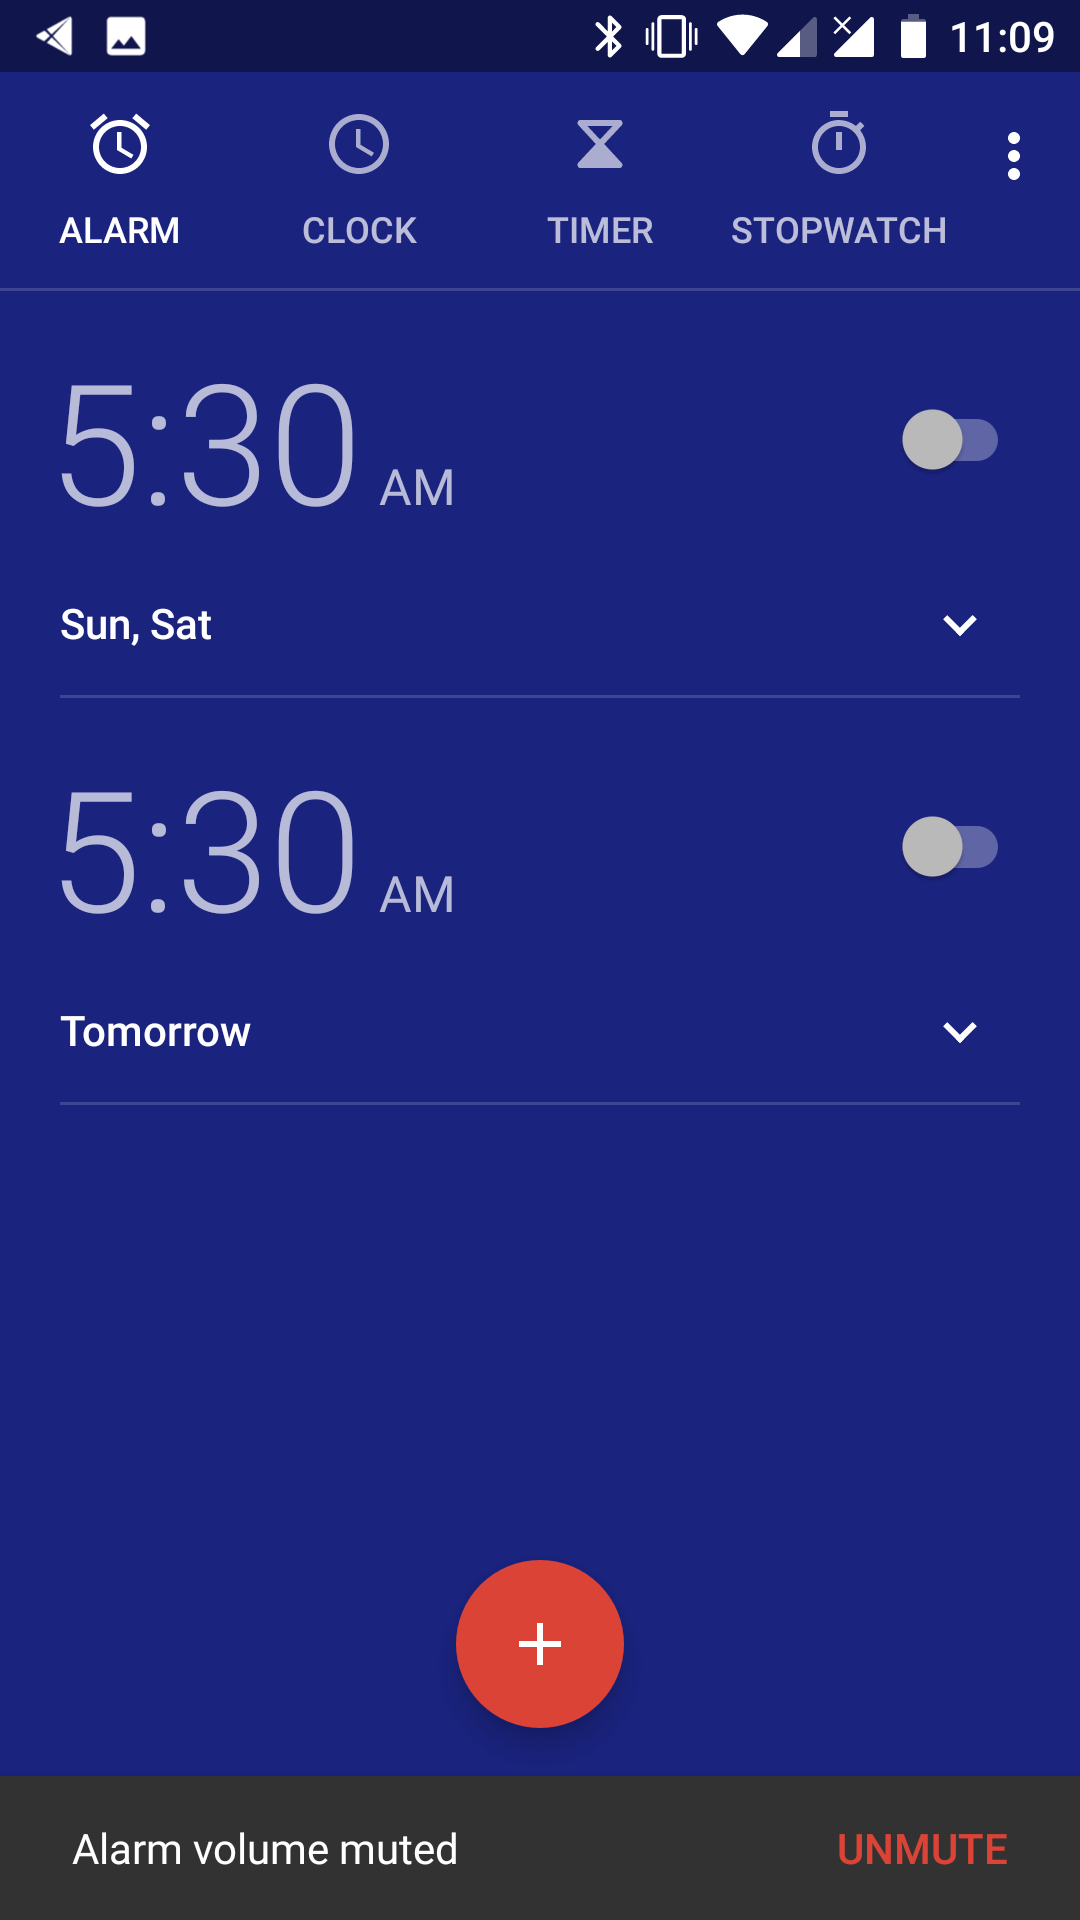
\includegraphics[scale=0.1]{volumemuted.png} Wszystkie ekrany aplikacji utrzymane są w podobnej kolorystyce, czcionka jest podobnej wielkości i kroju. Ponadto na różnych ekranach możemy się spodziewać podobnych gestów, które aplikacja od nas wymaga.\\
        \hline
        4. Poprawność zarządzania błędami & 5/5 & Przez cały okres używania aplikacji nie ujawnił się ani jeden błąd, więc zarządzaniu błędami przydzielam maksymalną ocenę.\\
        \hline
    \end{longtable}

    \subsection{Zadanie 3.4. Responsywność stron internetowych}

    Sprawdź czy serwisy badane w zadaniu 2.2 są responsywne

    \begin{longtable}{|p{0.33\textwidth}|p{0.33\textwidth}|p{0.33\textwidth}|}
        \textbf{Nazwa serwisu} & \textbf{Min. szerokość ekranu} & \textbf{Uwagi}\\
        \hline
        http://www.pollub.pl/ & Nie dotyczy & Strona nie jest responsywna w żadnym stopniu. Ani jeden element strony nie dostosowuje się do widoku mobilnego\\
        \hline
        http://www.nngroup.com/ & 320px &Strona jest responsywna, jednak na widoku mobilnym strona jest szersza niż szerokość ekranu w moim urządzeniu, przez co istnieje możliwość scrollowania w poziomie, co nagatywanie wpływa na UX\\
        \hline
        http://www.lublin.eu/ & 320px & Strona ta jest w pełni responsywna, na stronie głównej aktualności się dobrze dostosowują do mobilnego widoku, menu ładnie się prezentuje na widokach mobilnych też\\
        \hline
        http://www.biblioteka.pollub.pl/ & Nie dotyczy & Ta subdomena pollub także nie wykazuje żadnych elementów responsywności\\
        \hline
    \end{longtable}


\end{document}
